\def\year{2015}
%File: formatting-instruction.tex
\documentclass[letterpaper]{article}
\usepackage{aaai}
\usepackage{times}
\usepackage{helvet}
\usepackage{courier}
\frenchspacing
\setlength{\pdfpagewidth}{8.5in}
\setlength{\pdfpageheight}{11in}
\pdfinfo{
/Title (Insert Your Title Here)
/Author (Put All Your Authors Here, Separated by Commas)}
\setcounter{secnumdepth}{0}
\usepackage{amsmath}  
\DeclareMathOperator*{\argmin}{\arg\!\min} 
\DeclareMathOperator*{\argmax}{\arg\!\max} 
\usepackage{graphicx}
 \begin{document}
% The file aaai.sty is the style file for AAAI Press 
% proceedings, working notes, and technical reports.
%
\title{Inverse Reinforcement Learning from Failure}
% \author{AAAI Press\\
% Association for the Advancement of Artificial Intelligence\\
% 2275 East Bayshore Road, Suite 160\\
% Palo Alto, California 94303\\
% }
\maketitle
\begin{abstract}
\begin{quote}
In this paper, we approach the problem of Inverse Reinforcement Learning (IRL) from a rather different perspective. Instead of trying to only mimic an expert as in traditional IRL, we present a method that is capable of learning from data we would like to avoid. In particular, we propose a new IRL algorithm that extends the state-of-the-art method of Maximum Entropy Inverse Reinforcement Learning to exploit such failed demonstrations. Our experimental results show that learning in this fashion allows for better generalisation, especially in the presence of limited data.
\end{quote}
\end{abstract}

\section{Introduction}
	Inverse Reinforcement Learning (IRL) \cite{ng2000algorithms}, along with the closely related field of Inverse Optimal Control(IOC), have been subject to a steadily increasing amount of research. Solving the problem allows a machine to learn cost functionss for various decision making tasks, from human demonstration. This is in turn appealing for two reasons. Firstly it is especially fit for tasks that can be easily demonstrated whilst the cost function is hard to formalise, a classic example being car driving. Secondly, the output of the algorithm is a cost function, instead of a direct mapping to actions (a policy) which would fail when the configuration and dynamics of the environment change.\\
	All Inverse Reinforcement Learning methods to date focus on imitation of a certain type of behaviour. There are however, tasks for which we might have data that demonstrate behaviour that we would like to avoid. Consider for example tasks such as driving a car\cite{abbeel2004apprenticeship}. Since humans also learn this task by trial and error, demonstrations of both successful and failed behaviour are available, and labeling them as such is straightforward. Being able to learn in this fashion would be beneficial in a number of ways. Firstly, it would allow us to take into account more data, which is the main resource learning depends on. Secondly it would give us access to decisions, at areas of the state space, that do not exist within the demonstrations we would like to imitate. In this sense, the data is not only more, it is also more variable. Finally it would allow us to inject prior knowledge in the system through simulated data. For example if we want a robot not to hit obstacles, we would simulate the robot actually crashing, and then use that data to learn not to replicate the undesired behaviour. 

	 Starting from the principle of Maximum Entropy \cite{jaynes1957information} we first present a mathematical formulation that allows to learn useful reward functions from both behaviour that we want to match (successful) and behaviour that we want to avoid (failed). We first apply our theory to synthesised data, yielding results that demonstrate the ability of our algorithm to generalise better, in addition we demonstrate that the agent can learn to perform a task reasonably, simply by being told what to avoid. We go on to apply our method real robotic navigation data, again yielding superior results when compared to the state-of-the art.

	
\begin{figure}[t]
  \centering
  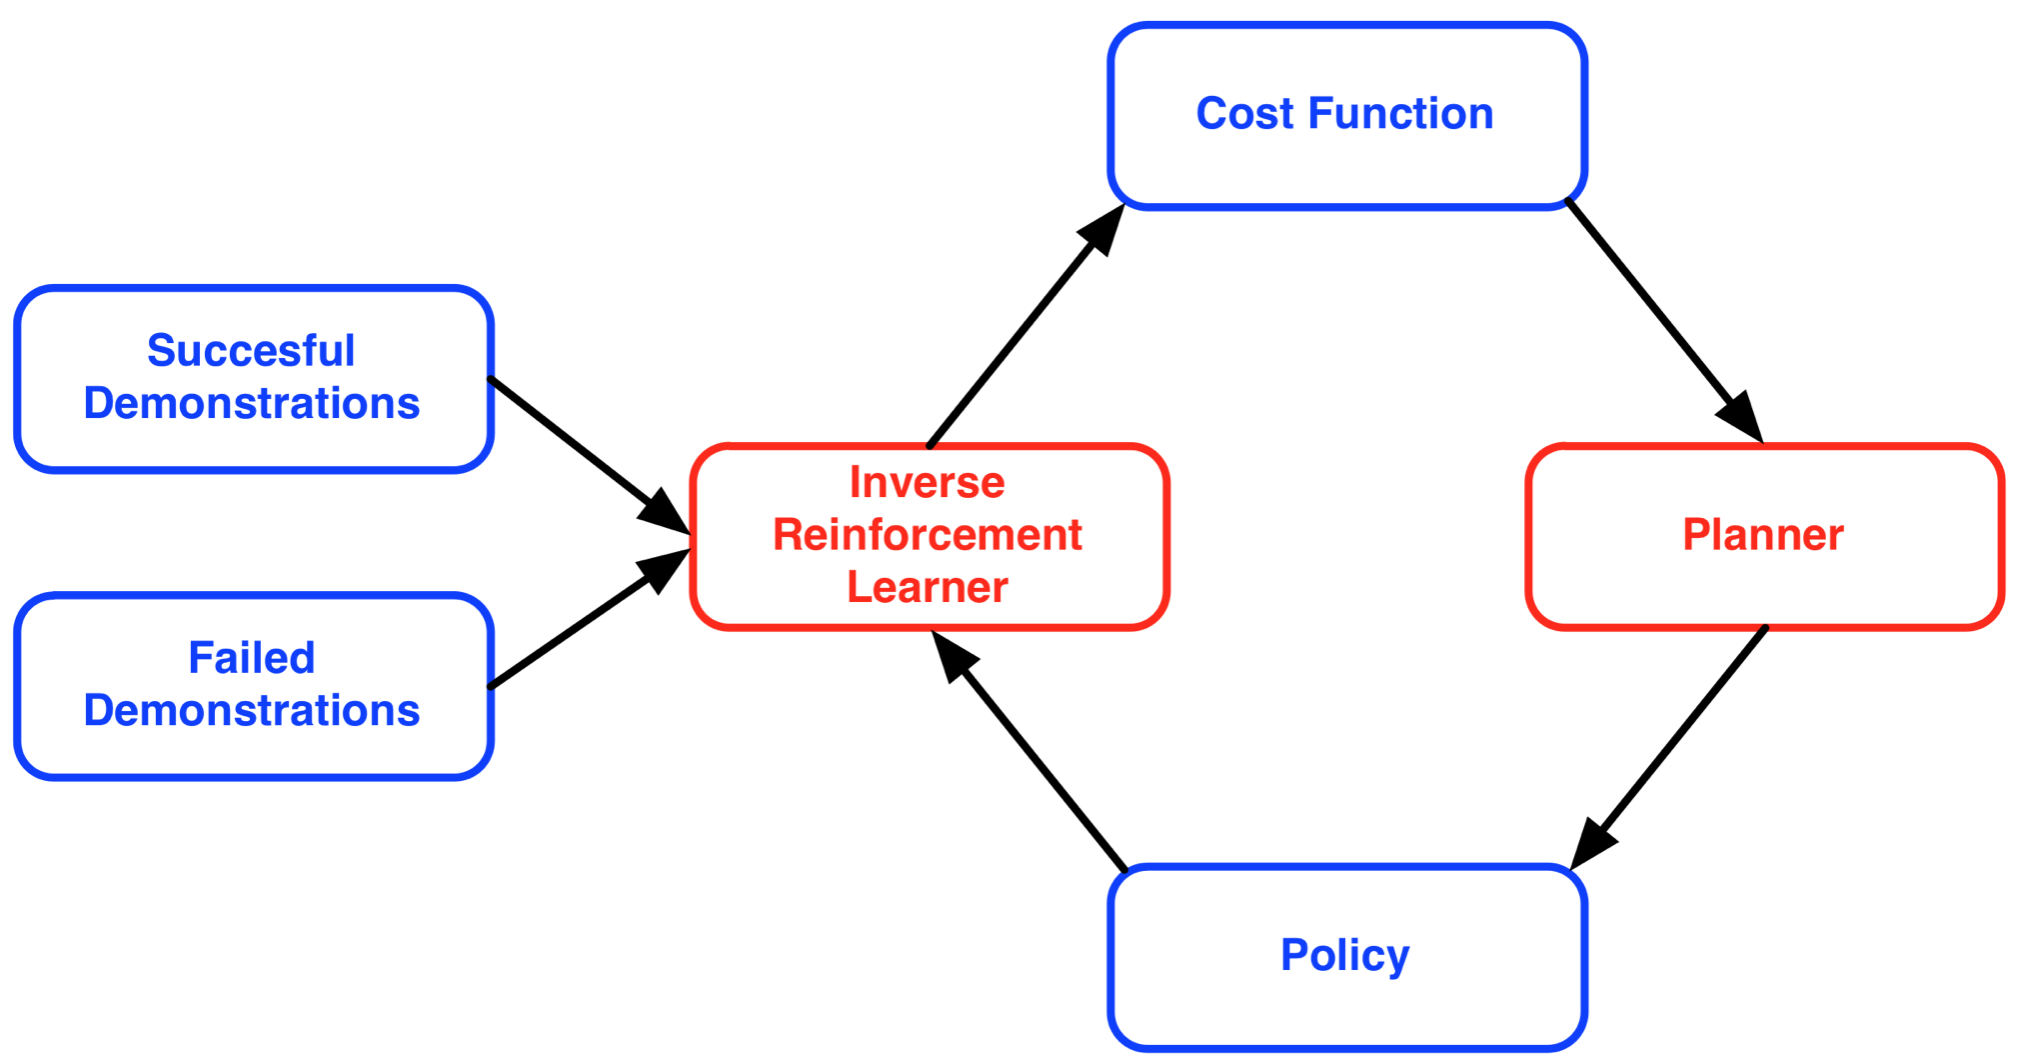
\includegraphics[width=0.9\columnwidth]{images/irlf.png}
  \caption{Method Outline 	\label{fig:IRLoutline}}
\end{figure}

\section{Background}
Figure \ref{fig:IRLoutline} outlines the general framework for IRL and IOC. An initial guess for our cost/reward function is input to the planner that produces a policy or a control law. Using this policy we can then simulate a decision making task from the same initial conditions as our dataset. By comparing the behaviour of our model with the data, we update the cost function. At convergence the behaviour of the model is similar what is observed in the data.
In the original as well as most of the susequent formulations of Inverse Reinforcement Learning, the planning phase in figure \ref{fig:IRLoutline} involves optimally solving a Markov Decision Process (MDP). An MDP is defined as a tuple $\langle\mathbf{S},\mathbf{A},\mathcal{T},R,\gamma\rangle$, where $\mathbf{S}$ and $\mathbf{A}$ are the sets of discreete states and actions respectively, $\mathcal{T}$ is a Transition function that maps a state ($s$) and an action ($a$) to the next state ($s'$), $R$ is a reward function and $\gamma$ is the discount factor. 
Optimally solving an MDP involved finding a policy $\pi(a,s) = P(a\,|\,s)$, that maximises the the expected (discounted) future rewards.

\begin{equation}
 V^\pi(s) = E\{\sum_{t = 0}^h \gamma^tR(s_t,a_t)\,\vert\, s_0 = s\}\quad,
\end{equation}

In IRL the $R$ is considered to be unknown and in its simplest form represented as a linear combinations of features:
\begin{equation}
R(s,a) = \sum_k^Kw_k\phi_k(s,a). \label{eq:rew}
\end{equation}
Which in turn gives rise to the parametrised Value function.

\begin{equation}
 	V^\pi(s) = w \cdot E\{\sum_{t = 0}^h \gamma^t\phi(s_t,a_t)\,\vert\, s_0 = s\}\quad,
\end{equation}

In adition to this parametrisation the algorithm is provided with a dataset ${\mathcal{D}}$ of $N$ trajectories $\zeta$ each of length $T_{\zeta_n}$ and consisting of state-action sequences from $\mathbf{S}$ and $\mathbf{A}$ respectively. The dataset can therefore be summarised as $\mathcal{D}:\big\{ \zeta_1,\zeta_2,...\zeta_N \big\}$ where $\zeta_n = \{(s^{\zeta_n}_1,a^{\zeta_n}_1),(s^{\zeta_n}_2,a^{\zeta_n}_2),...(s^{\zeta_n}_{T_{\zeta_n}},a^{\zeta_n}_{T_{\zeta_n}})\}$. 

A crucial quantity used by IRL algorithms, is the \emph{feature expectation} that describes the accumulation of features of the agent over time, and is related to the value through the unknnown weights $w$. 

\begin{equation}
 	\Phi_{\pi(s)} = \cdot E\{\sum_{t = 0}^h \gamma^t\phi(s_t,a_t)\,\vert\, s_0 = s\}\quad, \label{eqn:model_fe}
\end{equation}

From the dataset ${\mathcal{D}}$ we can derive a similar quantity as an empirical feature expectation:

\begin{equation}
	\widetilde{\Phi}_{\mathcal{D}} =\frac{1}{N}\sum_{\zeta\in\mathcal{D}}\sum_{t=0}^{T_{\zeta}}\phi(s^\zeta_t,a^\zeta_t). \label{eqn:empirical_fe}
\end{equation}

The aim of an inverse reinforcement learning algorithm is to find the configuration of weights $w$ that makes $\widetilde{\Phi}_{\mathcal{D}} = \Phi_{\pi(s)}$. 

Different algorithms cast the IRL problem to existing, mature and reliable frameworks such as structured prediction \cite{ratliff2006maximum} and Bayesian inference \cite{ramachandran2007bayesian}, while others rely on non-linear representation of the reward such as Gaussian processes \cite{levine2011nonlinear}, Neural Networks and Decision Trees\cite{ratliff2007boosting}. In this paper we will concentrate on two similar methods introduced by Ziebart in \cite{ziebart2008maximum} and \cite{ziebart2010modelingthesis} and cast the problem in terms of maximum entropy. Specifically they seek a policy $\pi(a,s)$ with maximum entropy, constrained to match the feature expectations between the data and the model. the first method is convex when the environment dynamics are deterministic, while the other is convex for stochastic environments as well. In these methods the planning is done using a soft version of the Bellman equation\cite{sutton1998reinforcement}. This outputs a stochastic policy, that is in turn used to generate the required feature expectations by simulating paths at the same initial conditions as those seen in the data. Finally the algorithm updates the weights using gradient descent. We will focus on the case of linear rewards, although extending the method using non-linear function approximators is straightforward.

	The principle of maximum entropy attempts to find the distribution that is maximally notcommittal to presence of missing information \cite{jaynes1957information} and forms an essential both of Ziebarts
	initial method as well as our extension. Formally the principle can be cast as an optimisation problem.

	\begin{equation}
	\argmax_{P(x)} -\sum_i^N p(x_i)\log(x_i)
	\end{equation}
	\begin{equation}
	\text{subject to:} \quad \sum_i^N p(x_i)f_k(x_i) = \widetilde{F}_k \quad \forall k \label{eqn:constraint1}
	\end{equation}
	\begin{equation}
	\text{and:} \quad \sum_i^N p(x_i) = 1 \label{eqn:constraint2}
	\end{equation}

	Where $x$ is a discrete random variable of N possible values, P(x) is the probability distribution over these values. The optimisation asks for the distribution that has maximum entropy, while constrained to produce function expectations $\sum_i^N p(x_i)f_k(x_i)$ that are consistent with the empirical function expectations $\widetilde{F}_k$ for all K of such functions.\\


\section{Method}
	Our method extends the original maximum entropy formulation, allowing the injection of further demands for our optimal distribution $P(x)^*$. Specifically we are interested in empirical function expectations $\widetilde{G}_k$ that we would like to keep away from. Modifying the original problem we have:  
	\begin{equation}
	\argmax_{P(x)} -\sum_i^N p(x_i)\log(x_i) + \frac{C}{2}\sum_k^K(\sum_i^N p(x_i)f(x_i) - G_k)^2
	\end{equation}
	

	\begin{equation}
	\text{subject to:} \quad \sum_i^N p(x_i)f_k(x_i) = \widetilde{F}_k \quad \forall k \label{eqn:match_constraint}
	\end{equation}

	\begin{equation}
	\text{and:} \quad \sum_i^N p(x_i) = 1
	\end{equation}
	Intuitively the loss function $\frac{C}{2}\sum_k^K(\sum_i^N p(x_i)f(x_i) - G_k)^2$ attempts to bias the 
	maximum entropy distribution by penalising distributions that yield feature expectations that are close 
	to those we know empirically should be avoided.\\
	Solving using the method of Lagrange multipliers first yields the Lagrangian.
\begin{equation}
	\begin{split}
	\mathcal{L}(P(x),\lambda,\mu) &=  -\sum_i^N p(x_i)\log(x_i) \\
	&+\frac{C}{2}\sum_k^K(\sum_i^N p(x_i)f(x_i) - G_k)^2\\
	 & + \sum_k^K\lambda_k(\sum_i^N p(x_i)f(x_i) - \widetilde{F}) + \mu(\sum_i^N p(x_i) - 1)
	\end{split}
\end{equation}
Which we differentiate with respect to the variables $p(x_n)$ and equate to 0.
\begin{equation}
	\begin{split}
	&\nabla_p(x_n)\mathcal{L} =  -\big(\log(p(x_n))+1\big) +\mu + \\
	&\sum_k^K f_k(x_n)\big(\lambda_k+C(\sum_i^N p(x_i)f(x_i) - G_k)\big)\\
	&p(x_n) =\exp \Big( \sum_k^Kf_k(x_n)\big(C\sum_i^N p(x_i)f(x_i) - G_k\\
	&+\lambda_k\big) + \mu \Big)
	\end{split}
\end{equation}
Unlike the original maximum entropy formulation we cannot determine $p(x_n)$ directly, instead 
we can use gradient descent or the iterative scheme:
\begin{equation}
p(x_n)_t =\exp \Big(\mu+ \sum_k^Kf_k(x_n)\big( C(\sum_i^N p(x_i)_{t-1}f(x_i) - G_k)+\lambda_k\big)\Big) \label{eqn:iter_scheme}
\end{equation}
After the maximisation of $\mathcal{L}$ with respect to the distribution, the term $\sum_i^N p(x_i)_{t-1}f(x_i) - G_k$ is a constant.
We can threfore define:
\begin{equation}
	\begin{split}
	p(x_n) =\exp \Big( \sum_k^K\big(D_k+\lambda_k\big)f_k(x_n) + \mu \Big)\\
	\text{where} \quad D_k = C\big(\sum_i^N p(x_i)f_k(x_i) - G_k\big)
	\end{split}
\end{equation}
Replacing the expression for $p(x_n)$ into equation \ref{eqn:constraint2}:
\begin{equation}
	\sum_i^N \exp \Big( \sum_k^K\big(D_k+\lambda_k\big)f_k(x_i) + \mu \Big) = 1
\end{equation}
\begin{equation}
	\mu = \ln Z(D,\lambda)
\end{equation}
Where $Z(D,\lambda)$, is our new partition function.
\begin{equation}
	Z(D,\lambda) = \sum_i^N \exp \Big( -\sum_k^K\big(D_k+\lambda_k\big)f_k(x_i) \Big) 
\end{equation}

In addition, the expectation matching constraint \ref{eqn:match_constraint} is satisfied in a similar way as the original 
Maximum entropy formulation

\begin{equation}
	\widetilde{F}_k = -\frac{\partial\ln Z(D,\lambda)}{\partial\lambda_k}
\end{equation}

It therefore follows that as long as we can find the terms $D_k$ we can perform 
this penalised maximum entropy computation as before.

\subsection{Application to Inverse Reinforcement Learning}
We would now like to use this concept of penalising certain 
statistical outcomes of our distribution, to learn to avoid certain behaviours.\\ 
In the classical inverse reinforcement learning task, we try to find the
weights ($\lambda$) such that the model generates similar feature expectations to the 
data. In practice this implies that the feature expectation constraint (\ref{eqn:constraint1}) is relplaced by expessions
\ref{eqn:model_fe} and \ref{eqn:empirical_fe}, i.e the model and data feature expectations. The Maximum Entropy and Maximum Causal Entropy algorithms by Ziebart
essentially solve the maximum entropy optimisation problem, where the distribution to be optimised
is the policy of the agent $\pi(a,s)$.

We now assume acceess to a dataset of \emph{failed} demonstrations $\mathcal{D}_f$.
using equation \ref{eqn:empirical_fe} we can calculate feature expectations for this data
which in our case will represent the quantity $\widetilde{G}_k$. Using the derivation above along with the
inference methods describes in \cite{ziebart2010modelingthesis} we can now learn a maximum entropy policy, that is 
constrained to match the expert demonstrations and penalised for yielding feature expectations that are close
to the ones observed in the failed demonstrations. Applying our previous derivation to IRL however does
has a significant computational drawback, which is that we should perform the iterative scheme in (\ref{eqn:iter_scheme})
which requires the repetitive evaluation of the policy which in turn involves solving a computationaly expensive Markov Decision Process. Since the original algorithm is also iterative, we could use the policy found in the
previous iteration of the algorithm in order to make an aproximation for the term $D_k$ in the derivation above. This means that
instead of peforming iterations of (\ref{eqn:iter_scheme}) until convergence, and then update the weights, we update the weights first
and the n use the previous policy to compute $D_k$ which will give us the next policy.

\section{Experiments}
\subsection{Moving Obstacle Gridworld}
Our first set of experiments consider a moving obstacle Gridworld domain, shown in figure \ref{fig:gridworld}.
In this domain an agent moves in an environment, containing a moving obstacle, that could be moving either vertically
or horizontally and a target that is stationary. The goal of the agent is to reach the target, while avoiding 
the obstacle. The learning agent or \emph{appretnice} is not familiar with the task, yet he is provided with some data coming from two other agents
each with different aims. The first of these agents is an \emph{expert} at the task, his reward function ($R_e = \lambda_e\phi(s,a)$) is large and negative
for being in the same cell as the obstacle, and it is large an possitive for reaching the target. The second agent is a
\emph{taboo} agent with a reward function $(R_t=\lambda_t\phi(s,a))$ that is positive for colliding with the obstacle. Since we know the reward functions used for learning, we can directly evaluate the properties of our method. \\
Our experiments in this domain involve choosing five random initial train and test states for our agents $b_{0_{test}}$,$b_{0_{train}}$ and generating data for 15 decision steps. We then use the data generated using $b_{0_{train}}$ to train the apprentice, resulting in a learned reward function, $R_a = \lambda_a\phi(s,a)$ and the apprentice policy $\pi(s,a)_a$. Using this policy we perform trajectories using the initial conditions in $b_{0_{test}}$. These trajectories produce feature expectations for the model, which when multiplied with either of the weight vectors $\lambda_e,\lambda_t$ will give us the accumulated value for those initial states based on the reward functions of either the expert or the taboo. In other words if the apprentice generates feature expectations $\Phi_{\pi(s,a)_a}$ the Value of the apprentice based on the expert reward function is simply $\lambda_e^T\Phi_{\pi(s,a)_a}$. In addition to the difference in value, we also measure the absolute difference of the learned policies between appretice and expert $(\pi(s,a)_e - \pi(s,a)_a)$ We repeat this procedure 20 times with different initial train and test conditions, and report the results in Table \ref{tab:results} , an example run is shown in figure \ref{fig:results}

\begin{figure}[t]
  \centering
  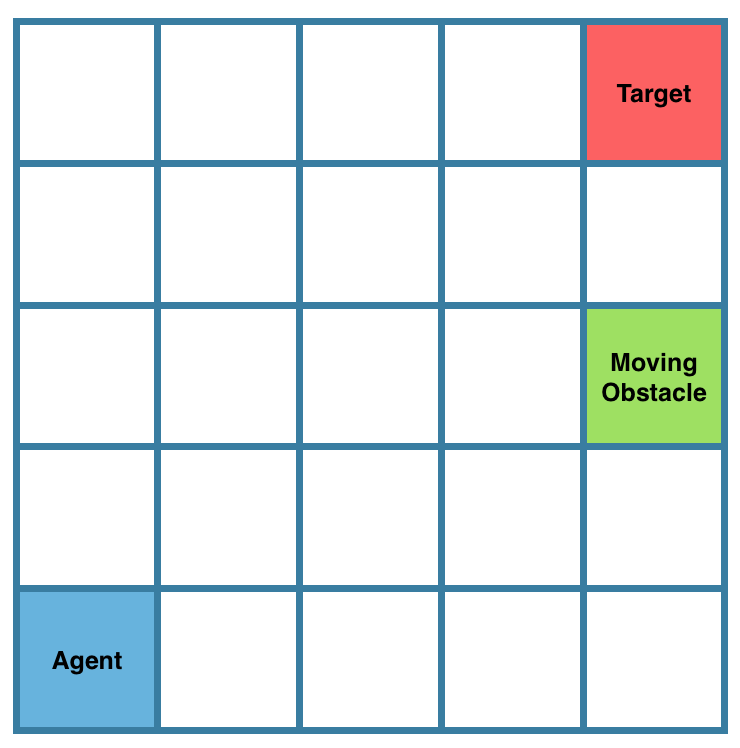
\includegraphics[width=0.5\columnwidth]{images/gridworld.png}
  \caption{Moving obstacle gridworld 	\label{fig:gridworld}}
\end{figure}
\begin{table}[]
\centering

\label{tab:results}
\begin{tabular}{|l|l|l|l|}
\hline
           & $\lambda_e(\Phi_{a}-\Phi_{e)}$& $\lambda_t(\Phi_{a}-\Phi_{t)}$ & $|\pi_a - \pi_t|$ (\%) \\ \hline
Original   & -6.125(2.06)        & 2.41(1.82)         & 15                    \\ \hline
Our Method & 0(0.2)              & 0.02(0.167)        & 10                    \\ \hline
\end{tabular}
\caption{Results on test set after 20 runs of random initial conditions. $\lambda_e$ represent reward weights, $\pi$ represents policy and $\Phi$ represents feature expectations. The subscripts $a,e,t$ represent the apprentice, expert and taboo agents respectively}
\end{table}
It should be apparent from the results, that using the additional data of avoidable behaviour allows the apprentice to 
come closer to the actual desired behaviour, which is that of the expert. Further more, in the third row of Table .. we can see that
even if the appretnice is trained only on the taboo agent, his policy and performance still come closer to the expert. This is further
evidence that learning to imitate and learning to avoid behaviours are related concepts and should be used interchangeable depending on the application.

\begin{figure}[t]
  \centering
  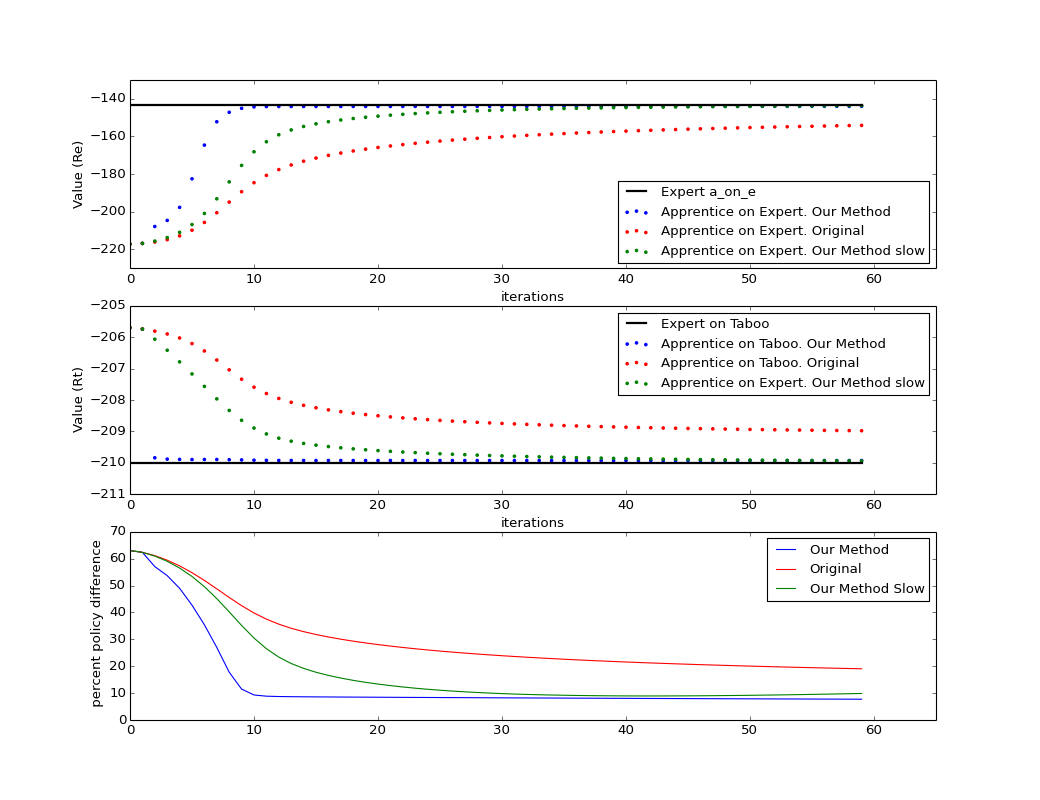
\includegraphics[width=0.9\columnwidth]{images/testgraph}
  \caption{A typical run for moving obstacle gridworld. Our method (blue) will quickly outperform the original algorithm. Achieving value that is closer to that of the expert, and reducing the difference with the desired policy\label{fig:results}}
\end{figure}

\subsection{Real Social Navigation Data.}




\section{Related Work}

Inverse Reinforcement Learning was introduced by \cite{ng2000algorithms} and \cite{abbeel2004apprenticeship}. The first probabilistic interpretation of the framework was introduced by Ramachandran and Amir 2007 and extended to Maximum Entropy IRL by Ziebart et al 2009. 	Learning from failure is an area that has found most attention in the Robotics community and specifically imitation learning. \cite{choi2015} introduces leveraged non stationary gaussian processes, that fit good data points while trying to avoid bad ones. The method was also applied to robotic navigation, but not in terms of IRL. \cite{grollman2012robot} Use past failures of the robot to initialise robot policies, and conclude that there is indeed information in failed trajectories that should not be discarted. IRL has been previously applied to social robot navigation, notable works are those of \cite{henry2010learning} and \cite{vasquez2014inverse}, that use pedestrian simulators to extract the undelying reward function of a human controller. To our knowledge our work is the first to implement Learning from Failure in Inverse Reinforcement Learning and assess its performance using real social navigation data.
\section{Conclusions and Future Work}
In this paper we have introduced a new framework for Inverse Reinforcement Learning that allows an agent to not only imitate certain behaviours but to also avoid others. The benefits this approach is that it allows otherwise useless data to be used and further enables a designer to inject prior information in the learning, by specifying, through simulated data, what behaviours should be avoided. We have derived a theoretically sound method by directly modifying the derivation of the Maximum Entropy and carying that through to MaxEnt IRL, providing solutions to the computational obstacles that arise. We have further performed exhaustive experiments in a toy domain, that clearly demonstrate that our method can generalise much better that the baseline IRL algorithm. Finally we have performed learning on real data, again showing that our method is superior to the baseline.  

\bibliographystyle{aaai}
\bibliography{references}




	
\end{document}
